\PassOptionsToPackage{unicode}{hyperref}
\PassOptionsToPackage{hyphens}{url}

\documentclass{article}

\usepackage[T1]{fontenc}
\usepackage[utf8]{inputenc}

\usepackage{xcolor}
\usepackage{amsmath,amssymb}
\usepackage{algorithm}
\usepackage{algpseudocode}
\usepackage{graphicx}
\usepackage{float}
\usepackage{longtable,booktabs,array}
\usepackage{calc}
\usepackage{etoolbox}
\IfFileExists{microtype.sty}{\usepackage{microtype}}{}
\usepackage{hyperref}
\usepackage{bookmark}
\IfFileExists{xurl.sty}{\usepackage{xurl}}{} % safer than unconditional
\urlstyle{same}
\setcounter{secnumdepth}{3}
\setlength{\emergencystretch}{3em}
% --- Fix unicode chars that break pdfLaTeX (arXiv-friendly) ---
\usepackage{newunicodechar}
\newunicodechar{≤}{$\le$}
\newunicodechar{≥}{$\ge$}
\newunicodechar{≈}{$\approx$}
\newunicodechar{±}{$\pm$}
\newunicodechar{Θ}{$\Theta$}
\newunicodechar{Ω}{$\Omega$}
\newunicodechar{ω}{$\omega$}
\newunicodechar{ρ}{$\rho$}
\newunicodechar{Σ}{$\Sigma$}

\makeatletter
\patchcmd\longtable{\par}{\if@noskipsec\mbox{}\fi\par}{}{}
\makeatother

\hypersetup{
  pdftitle={LadderSort: Adaptive Subsequence-Based Sorting Algorithm},
  hidelinks,
  pdfcreator={LaTeX}
}

\title{LadderSort: Adaptive Sorting via Interleaved Nondecreasing Subsequences}

\author{%
  Malik Mir Hamza Nayab\textsuperscript{1}\thanks{Email: \href{mailto:hamza.nayab48@gmail.com}{hamza.nayab48@gmail.com}} \and
  Ghanwa Batool\textsuperscript{2}\thanks{Email: \href{mailto:ghanwa@cuiatd.edu.pk}{ghanwa@cuiatd.edu.pk}}\\[0.5em]
  \textsuperscript{1,2}Comsats University Islamabad, Abbottabad Campus, Pakistan
}

\date{}

\begin{document}
\maketitle

\begin{abstract}
Many real-world workloads produce sequences that are not globally sorted but are interleavings of several ordered streams. 
We present \emph{LadderSort}, a deterministic adaptive comparison sort whose running time depends on the number \(K\) of interleaved nondecreasing subsequences in the input. LadderSort performs (i) a single left-to-right pass that assigns each key to the leftmost subsequence whose tail is \(\le\) the key, using a locality-aware hinted search over a nonincreasing tail array, followed by (ii) an adaptive merge: direct return for \(K=1\), a two-way galloping merge for \(K=2\), and a fixed loser-tree merge for \(K>2\). The resulting running time is \(O(N\log K)\) with \(O(N+K)\) auxiliary space. Equal keys are resolved deterministically via a fixed ladder-identifier tie-break during merging, yielding reproducible behavior under duplicates but not guaranteeing global stability across ladders. Experiments on arrays of up to \(10^8\) 32-bit integers demonstrate speedups of up to \(1.7\times\) over TimSort on interleaved-stream workloads with small \(K\), while remaining competitive on uniform random inputs and exhibiting the expected worst case on strictly descending inputs.
\end{abstract}

\noindent\textbf{Keywords:} adaptive sorting; nondecreasing subsequences; multiway merge; loser tree; presortedness; streaming data; performance evaluation

\newpage

\section{Introduction}

Sorting is a fundamental primitive in computing systems, underpinning database operators, stream processing pipelines, search indexing, analytics, and online services. Classical comparison-based algorithms such as mergesort, quicksort, and heapsort provide robust worst-case guarantees, but their performance is typically characterized by \(\Theta(N\log N)\) regardless of whether the input contains latent order. Practical implementations therefore incorporate adaptivity. A prominent example is TimSort, which detects contiguous monotone runs during a linear scan and merges them using carefully engineered policies. This approach is highly effective when the input contains long sorted segments, but it is less well matched to workloads in which order is present but noncontiguous.

\paragraph{Paper story.}
The central idea of this paper is that many modern workloads contain order that is not contiguous but \emph{interleaved}. 
While algorithms such as TimSort adapt to the number and length of contiguous runs, LadderSort adapts to a different structural parameter: the number \(K\) of interleaved nondecreasing subsequences in the input. 
LadderSort performs a deterministic tail-guided decomposition that reconstructs these subsequences during a single scan, followed by an adaptive merge whose cost scales with \(K\). 
As a result, the running time becomes \(O(N\log K)\), meaning performance depends on the amount of interleaved structure present rather than solely on \(N\) or the number of contiguous runs. 
This makes LadderSort particularly effective for fan-in workloads where multiple ordered streams are interleaved, such as feed aggregation, telemetry pipelines, and index merges.

In many modern systems, data arrives as a fan-in of multiple sources that are individually ordered but interleaved in time. Examples include social-feed assembly from multiple producers, market-data aggregation from multiple venues, telemetry ingestion from distributed sensors, and partial index or posting-list merges in search engines. These workloads often exhibit short alternations and bursty interleavings that fragment contiguous runs, even though the global sequence can be viewed as an interleaving of only a small number of nondecreasing streams. Under such conditions, run-adaptive methods may observe many short runs and incur additional merge scheduling and comparison overhead, while failing to exploit the deeper interleaved structure.

This paper introduces \emph{LadderSort}, a deterministic sorting algorithm designed to target fan-in structure directly. Instead of adapting to the number and lengths of contiguous runs, LadderSort adapts to a structural parameter \(K\): the number of nondecreasing subsequences produced by a deterministic tail-guided decomposition. The algorithm proceeds in two phases. In Phase~1, a single left-to-right scan assigns each element to the leftmost subsequence whose tail is less than or equal to it, maintaining an array of subsequence tails in nonincreasing order. To reduce placement overhead in practice, the implementation employs a locality-aware hinted search that combines constant-time probing near the previous placement, exponential galloping to bound the search interval, and binary search within that interval. In Phase~2, the resulting subsequences are merged using a strategy selected by \(K\): direct return when \(K=1\), a two-way galloping merge when \(K=2\), and a fixed loser-tree merge when \(K>2\).

This design yields a running time of \(O(N\log K)\) with \(O(N+K)\) auxiliary space. When \(K=1\), LadderSort runs in linear time; as \(K\) increases, the cost degrades smoothly toward \(O(N\log N)\). The implementation specifies deterministic handling of duplicates: during multiway merge, equal keys are ordered by increasing ladder identifier. This rule ensures reproducible output under heavy duplicate plateaus common in timestamped streams, while not guaranteeing global stability with respect to original input order across ladders.

\noindent\textbf{Contributions.}
\begin{itemize}
\item We introduce \emph{LadderSort}, an adaptive comparison sort whose complexity depends on the number \(K\) of interleaved nondecreasing subsequences in the input rather than on contiguous runs alone.
\item We present a deterministic tail-guided decomposition that constructs these subsequences during a single scan while maintaining a nonincreasing array of subsequence tails.
\item We design an adaptive merge phase that selects between direct return, two-way galloping merge, and deterministic loser-tree \(K\)-way merge.
\item We experimentally evaluate the algorithm on datasets up to \(10^8\) elements and show that it provides substantial speedups on interleaved-stream workloads where \(K\) is small, while remaining competitive on unstructured inputs.
\end{itemize}

\section{Related Work}\label{related-work}

\subsection{General-Purpose Comparison Sorts}\label{general-purpose-comparison-sorts}

Textbook comparison-based sorting algorithms such as mergesort, quicksort, heapsort, and their hybrids (for example introsort, pattern-defeating quicksort, and BlockQuicksort) target robust worst-case guarantees and good constants on a wide range of inputs, but they do not explicitly parameterize cost by latent order beyond simple pivot or run heuristics \([1,15\text{--}17]\). Pattern-defeating quicksort strengthens introsort's defenses against adversarial patterns and small-distinct-key cases, while BlockQuicksort reduces branch mispredictions using blocked partitioning \([15,16]\).

A classic “best-of-both-worlds” alternative is \emph{Smoothsort} (Dijkstra), an in-place heapsort variant that achieves \(O(n)\) time on already sorted inputs while preserving \(O(n\log n)\) worst-case behavior \([2]\). Smoothsort is adaptive in the sense of speeding up on presorted data, but it does not explicitly exploit the case where the input is an interleaving of a small number of sorted streams (small \(K\)), which is the target regime for LadderSort.

\subsection{Run-Adaptive Natural Merges}\label{run-adaptive-natural-merges}

A large body of work exploits contiguous monotone runs discovered during a left-to-right scan (natural mergesort). TimSort is the most widely deployed variant; it detects ascending or descending runs, applies galloping, and controls merge order via stack invariants. Formal analyses bound its complexity by \(O(n\log n)\) in the worst case and \(O(n\log \rho)\) as a function of the number of runs \(\rho\) \([3]\).

\paragraph{Merge policies (PowerSort and variants).}
Subsequent work has improved merge scheduling---the policy that decides which runs to merge and when. PowerSort (and its multiway extension) selects near-optimal merge orders with negligible overhead and has influenced industrial implementations (including CPython’s list sort) \([4,5]\). AdaptiveShiversSort proposes alternative policies with \(nH + O(n)\) style bounds, where \(H\) is an entropy measure over run lengths \([6]\). These designs adapt to contiguous order: when inputs alternate frequently (large \(\rho\)) but consist of only a few nondecreasing subsequences, they can still observe many short runs and incur extra merge-scheduling overhead. LadderSort is complementary: it adapts to a noncontiguous fan-in parameter (\(K\)) rather than to the run count \(\rho\).

\subsection{Measures of Presortedness and Adaptive Sorting}\label{measures-of-presortedness}

Classical adaptive-sorting theory studies algorithmic cost as a function of disorder measures such as runs, inversions, oscillations, exchanges, and entropy. Foundational results formalize axioms for such measures and provide lower bounds and algorithms that are optimal with respect to specific measures \([7,8]\).

\paragraph{Encroaching lists.}
Skiena’s \emph{encroaching lists} technique provides both (i) a presortedness measure and (ii) a practical way to build a small family of monotone subsequences by inserting each element into one of two ends of existing lists \([9]\). This is closely related in spirit to LadderSort’s Phase~1: both construct multiple monotone subsequences that summarize latent order beyond contiguous runs. The key distinction is that LadderSort uses a deterministic tail-guided placement rule aligned with the leftmost feasible ladder (Definition~3) and then explicitly performs an adaptive multiway merge whose cost scales as \(O(n\log K)\).

\subsection{Sequence Decomposition and LIS/LDS Connections}\label{sequence-decomposition}

Patience sorting and chain decomposition provide a structural lens on sequence order. The minimum number of nondecreasing subsequences into which a sequence can be partitioned equals the length of a longest decreasing subsequence (LDS), a corollary of Dilworth's theorem for permutation posets \([10\text{--}12]\). Practical LIS routines maintain an array of pile tops and place each element by binary search in \(O(\log K)\) time, where \(K\) is the number of piles \([10]\). LadderSort borrows this tail-guided placement (augmented with locality-friendly hints and galloping) but, unlike LIS algorithms, retains all subsequences and completes the sort via a final \(K\)-way merge. This ties the algorithmic cost \(O(n\log K)\) directly to a classical structural parameter.

\subsection{Multiway Merging and Tournament/Loser Trees}\label{multiway-merging}

Tournament trees and their loser-tree variant are classical data structures for multiway merging. They support \(K\)-way merge in \(O(\log K)\) per extract after \(O(K)\) build time and are widely used in external-memory and streaming contexts \([1,13,14,17]\).

\section{Materials and Methods}\label{materials-and-methods}

\subsection{Methodology Overview}\label{methodology-overview}

The proposed algorithm is named LadderSort because it inserts each element step-by-step into an assigned subsequence (a \emph{ladder}). It operates in two phases: decomposition into ladders, followed by an adaptive merge.

\begin{figure}[H]
\centering
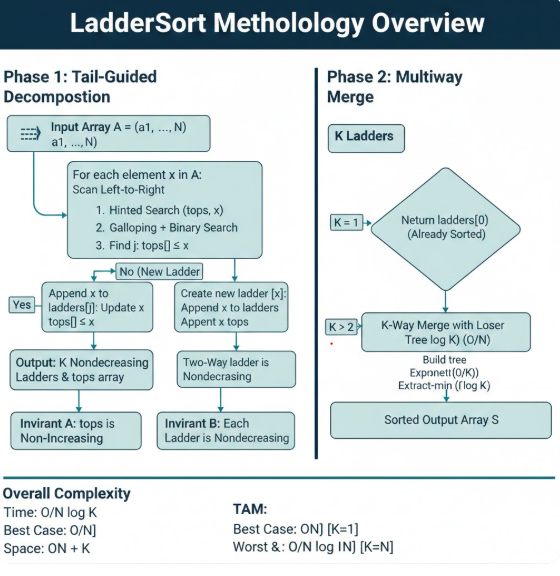
\includegraphics[width=0.85\linewidth]{media/media/image1.png}
\caption{Methodology overview of LadderSort.}
\label{fig:overview}
\end{figure}

\subsection{Two-Phase Description}\label{two-phase}

\paragraph{Phase 1 (decomposition).}
As the input array is traversed from left to right, elements are grouped into nondecreasing subsequences (ladders). For each ladder, the last element is its \emph{tail}. All tails are stored in a separate array \texttt{tops}, kept in nonincreasing order. When processing a new element \(x\), the algorithm searches \texttt{tops} using an initial galloping step to bound the search interval, then binary search to locate the first tail \(\le x\). If \(x\) is smaller than all tails, a new ladder is created. This produces multiple sorted subsequences.

\paragraph{Phase 2 (merge).}
Once all ladders have been created, the number \(K\) determines the merge strategy. If \(K=1\), the ladder is returned directly. If \(K=2\), a two-way merge with galloping is used. If \(K>2\), a \(K\)-way merge based on a loser tree is used. This design adapts to \(K\), achieving best-case time \(O(N)\) when the input is already sorted and worst-case time \(O(N\log N)\) when \(K\) is on the order of \(N\).


\section{Algorithm (Formal Definition)}
\label{sec:algorithm}

\subsection{\textbf{Problem Setting and Notation}}
Let $A = \langle a_1, a_2, \dots, a_N\rangle$ be a sequence of keys drawn from a totally ordered domain $(\mathcal{D}, \le)$.
We write $[m] := \{1,2,\dots,m\}$.
The goal is to output a sequence $S$ that is a nondecreasing permutation of $A$.

\paragraph{Deterministic tie handling (implementation).}
Our implementation sorts plain keys and resolves equal-key comparisons deterministically.
In Phase~1 (decomposition), placement uses the predicate ``$\texttt{tops}[j] \le x$''; since $x$ is appended to exactly one ladder, each ladder remains nondecreasing.
In Phase~2 (merge), comparisons use the key order first, and when keys are equal, we apply a fixed tie-break rule based on ladder identifier (Definition~5). This makes the algorithm deterministic on inputs with duplicates, but it does not enforce global stability with respect to the original input order across different ladders.


\subsection{\textbf{Ladders and the Parameter $K$}}

\paragraph{Definition 1 (Ladder).}
A \emph{ladder} is a finite sequence $L=\langle \ell_1,\dots,\ell_m\rangle$ such that
\[
\ell_1 \le \ell_2 \le \cdots \le \ell_m,
\]
i.e., $L$ is nondecreasing under the key order $\le$.


\paragraph{Definition 2 (Tail and tail array).}
Given a nonempty ladder $L$, its \emph{tail} is $\mathrm{tail}(L) := \ell_m$.
During Phase~1 the algorithm maintains:
\begin{itemize}
\item a list of ladders $(L_1,\dots,L_K)$, and
\item an array $\texttt{tops}[1..K]$ where $\texttt{tops}[j] := \mathrm{tail}(L_j)$.
\end{itemize}
The algorithm maintains the invariant:
\[
\texttt{tops}[1] \ge \texttt{tops}[2] \ge \cdots \ge \texttt{tops}[K].
\]
(With $\ge$ understood as the reverse of the comparison order in use.)

\paragraph{Definition 3 (Placement index).}
For a key $x$ and a nonincreasing array $\texttt{tops}[1..K]$, define the placement index
\[
\pi(x; \texttt{tops}) := \min\{ j \in [K] : \texttt{tops}[j] \le x \},
\]
if the set is nonempty; otherwise define $\pi(x;\texttt{tops}) := K+1$.

\paragraph{Definition 4 (Formal definition of $K$).}
Let $(L_1,\dots,L_K)$ be the ladders constructed by Phase~1 using the placement rule in Definition~3.
Then $K$ is the \emph{number of ladders produced by this deterministic construction} (equivalently, $K = |\texttt{tops}|$ at the end of Phase~1).
Note that this $K$ is algorithm-induced; it is not assumed to be the minimum possible number of nondecreasing subsequences.

\subsection{\textbf{Phase 1: Tail-Guided Decomposition}}

\paragraph{Invariant (Phase 1).}
After processing the prefix $\langle a_1,\dots,a_t\rangle$, the algorithm maintains:
(i) each $L_j$ is a ladder (nondecreasing),
(ii) $\texttt{tops}[j]=\mathrm{tail}(L_j)$, and
(iii) $\texttt{tops}$ is nonincreasing.

\begin{algorithm}[H]
\caption{\textsc{LadderSort}$(A)$ (formal)}
\label{alg:laddersort}
\begin{algorithmic}[1]
\Require $A=\langle a_1,\dots,a_N\rangle$
\Ensure Sorted sequence $S$
\State Initialize an empty list of ladders $(L_1,\dots,L_K)$ with $K\gets 0$
\State Initialize empty array $\texttt{tops}$
\State $\texttt{lastIdx} \gets 1$ \Comment{hint for locality; arbitrary when $K=0$}
\For{$i = 1$ to $N$}
    \State $x \gets a_i$
    \State $j \gets \textsc{HintedLowerBoundNonIncreasing}(\texttt{tops}, x, \texttt{lastIdx})$
    \Comment{$j$ returns $\pi(x;\texttt{tops})$ in Definition~3}
    \If{$j = K+1$}
        \State $K \gets K+1$
        \State $L_K \gets \langle x\rangle$
        \State $\texttt{tops}[K] \gets x$
    \Else
        \State Append $x$ to the end of $L_j$
        \State $\texttt{tops}[j] \gets x$
    \EndIf
    \State $\texttt{lastIdx} \gets j$
\EndFor
\State \Return \textsc{MergeByK}$(L_1,\dots,L_K)$
\end{algorithmic}
\end{algorithm}

\paragraph{Implementation note (search).}
\textsc{HintedLowerBoundNonIncreasing} returns the first index $j$ such that $\texttt{tops}[j]\le x$ (or $K+1$ if none exists).
Our implementation combines a constant-time local probe around the previous index, exponential galloping to bound the search interval, and a binary search within the bounded interval.

\subsection{\textbf{Phase 2: Merge and Formal Tie-Breaking}}

\paragraph{Definition 5 (Run identifier tie-break).}
For $K$ ladders, assign each ladder a fixed identifier $j\in[K]$ according to creation order.
During $K$-way merge, we compare current head elements of ladders by the total order:
\[
(x,j) \prec (y,\ell) \iff (x<y)\ \lor\ (x=y\ \wedge\ j<\ell).
\]
This makes the merge deterministic; equal keys are emitted by increasing ladder id.

\paragraph{Remark (stability).}
With the tie-break of Definition~5, equal keys are emitted in increasing ladder-id order, which is deterministic.
However, because equal keys from different ladders are ordered by ladder id (not by original input position), this implementation is not globally stable with respect to the original input order across ladders.


\begin{algorithm}[H]
\caption{\textsc{MergeByK}$(L_1,\dots,L_K)$}
\label{alg:mergebyk}
\begin{algorithmic}[1]
\Require Ladders $L_1,\dots,L_K$ (each nondecreasing)
\Ensure Sorted merge $S$
\If{$K=0$} \State \Return $\langle\rangle$ \EndIf
\If{$K=1$} \State \Return $L_1$ \EndIf
\If{$K=2$} \State \Return \textsc{TwoWayMergeWithGalloping}$(L_1,L_2)$ \EndIf
\State \Return \textsc{KWayMergeLoserTree}$(L_1,\dots,L_K)$ \Comment{uses Definition~5}
\end{algorithmic}
\end{algorithm}

\paragraph{Loser-tree merge (formal comparison).}
The loser-tree maintains one current head element per ladder.
At each step it outputs the globally smallest head under the comparison of Definition~5, advances that ladder, and restores the tournament structure in $O(\log K)$ time per output.

\subsection{\textbf{Complexity}}
Phase~1 performs $N$ placements, each costing $O(\log K)$ worst-case, yielding $O(N\log K)$ time.
Phase~2 costs $O(N)$ for $K\in\{1,2\}$ and $O(N\log K)$ for $K>2$ (after $O(K)$ initialization).
Auxiliary space is $O(N+K)$ to store ladders and merge state.

\section{\textbf{Correctness Proof}}
\label{sec:correctness}

We prove that \textsc{LadderSort} outputs a globally nondecreasing permutation of the input.
Throughout, ``sorted'' means nondecreasing under the key order $\le$.
When duplicates occur, Phase~2 uses the deterministic tie-break of Definition~5; this does not change
key-sortedness (it only selects a deterministic order among equal keys).

\subsection{\textbf{Lemma 1: Each ladder remains sorted}}
\label{lem:ladder_sorted}

\paragraph{Lemma 1.}
After processing any prefix $\langle a_1,\dots,a_t\rangle$ in Phase~1, every ladder $L_j$ is nondecreasing.

\paragraph{Proof.}
We argue by induction on $t$.
For $t=1$, the algorithm creates $L_1=\langle a_1\rangle$, which is trivially nondecreasing.
Assume the claim holds after processing $\langle a_1,\dots,a_{t-1}\rangle$.
At step $t$, the algorithm processes $x=a_t$ and chooses an index
$j=\pi(x;\texttt{tops})$ (Definition~3), i.e., the first $j$ such that $\texttt{tops}[j]\le x$,
or creates a new ladder if none exists.
If a new ladder is created, it is $\langle x\rangle$ and is sorted.
Otherwise, $x$ is appended to $L_j$ whose current tail is $\texttt{tops}[j]$.
By the choice of $j$, $\texttt{tops}[j]\le x$, so the new last two elements satisfy
$\mathrm{tail}(L_j)\le x$, preserving nondecreasing order of $L_j$.
All other ladders are unchanged and remain sorted by the induction hypothesis.
\hfill$\square$

\subsection{\textbf{Lemma 2: \texttt{tops} remains non-increasing}}
\label{lem:tops_nonincreasing}

\paragraph{Lemma 2.}
After each insertion step of Phase~1, the array $\texttt{tops}[1..K]$ is nonincreasing:
$\texttt{tops}[1]\ge \texttt{tops}[2]\ge \cdots \ge \texttt{tops}[K]$.

\paragraph{Proof.}
Assume $\texttt{tops}$ is nonincreasing before processing $x$.
Let $j=\pi(x;\texttt{tops})$.
There are two cases.

\emph{Case 1:} $j=K+1$ (no index satisfies $\texttt{tops}[j]\le x$).
Then $x<\texttt{tops}[p]$ for all $p\in[K]$, and the algorithm appends a new entry
$\texttt{tops}[K+1]\gets x$.
Thus $\texttt{tops}[K]\ge x=\texttt{tops}[K+1]$, preserving nonincreasing order.

\emph{Case 2:} $j\in[K]$.
The algorithm updates only $\texttt{tops}[j]\gets x$.
By definition of $\pi(\cdot)$, for all $p<j$ we have $\texttt{tops}[p]>x$, hence $\texttt{tops}[p]\ge \texttt{tops}[j]$ after update.
Also, since $j$ is the \emph{first} index with $\texttt{tops}[j]\le x$, we have for $j+1\le q\le K$:
$\texttt{tops}[q]\le \texttt{tops}[j]_{\text{old}}\le x=\texttt{tops}[j]_{\text{new}}$,
so $\texttt{tops}[j]\ge \texttt{tops}[q]$ holds after the update.
All other positions are unchanged.
Therefore $\texttt{tops}$ remains nonincreasing.
\hfill$\square$

\subsection{\textbf{Lemma 3: Merge outputs a globally sorted list}}
\label{lem:merge_sorted}

\paragraph{Lemma 3.}
Assume $L_1,\dots,L_K$ are nondecreasing ladders (Lemma~\ref{lem:ladder_sorted}).
Then \textsc{MergeByK}$(L_1,\dots,L_K)$ outputs a sequence $S$ that is globally nondecreasing
and is a permutation of the multiset union of the ladder elements.

\paragraph{Proof.}
We consider the cases in Algorithm~\ref{alg:mergebyk}.

\emph{Case $K=0$:} output is empty, trivially sorted and a permutation.

\emph{Case $K=1$:} output is $L_1$, which is sorted by assumption and is exactly the input multiset.

\emph{Case $K=2$:} \textsc{TwoWayMergeWithGalloping} is a standard two-way merge
(possibly accelerated by galloping) that repeatedly outputs the smaller current head
between the two sorted inputs. Galloping only skips ahead by outputting contiguous blocks that are
provably $\le$ the opposing head; it does not change correctness, only reduces comparisons.
Thus the result is sorted and contains each element exactly once.

\emph{Case $K>2$:} \textsc{KWayMergeLoserTree} maintains one current head per ladder and repeatedly
outputs the minimum head under the total order of Definition~5:
$(x,j)\prec(y,\ell)$ iff $x<y$ or ($x=y$ and $j<\ell$).
Because each ladder is nondecreasing, advancing a ladder pointer never decreases its current head.
At each step, the algorithm outputs the globally smallest available head (under $\prec$),
then advances exactly that ladder by one element and restores the tournament in $O(\log K)$ time.
Therefore the produced sequence is nondecreasing under $\prec$.
In particular, it is nondecreasing by key order $\le$, since $\prec$ refines $\le$ by only breaking ties.
Finally, every output step removes exactly one element from exactly one ladder, and the process
terminates after outputting all ladder elements, so the output is a permutation of the union.
\hfill$\square$

\subsection{\textbf{Lemma 4: Complexity is $O(N\log K)$}}
\label{lem:complexity}

\paragraph{Lemma 4.}
Let $N$ be the input length and let $K$ be the number of ladders produced in Phase~1.
Then \textsc{LadderSort} runs in $O(N\log K)$ time and uses $O(N+K)$ auxiliary space.

\paragraph{Proof.}
Phase~1 performs $N$ placements. Each placement computes
$j=\pi(x;\texttt{tops})$ using \textsc{HintedLowerBoundNonIncreasing}.
In the worst case, the search performs a bounded exponential gallop and a binary search
over an interval of $\texttt{tops}$, which costs $O(\log K)$ comparisons.
Thus Phase~1 costs $O(N\log K)$ time.

Phase~2 depends on $K$.
If $K\in\{0,1\}$ the return is $O(N)$.
If $K=2$, a standard merge outputs $N$ elements in $O(N)$ time.
If $K>2$, the loser tree builds in $O(K)$ time and performs $N$ extract-and-advance steps,
each costing $O(\log K)$, for total $O(K+N\log K)=O(N\log K)$ (since $K\le N$ always holds here).
Space: the ladders store all $N$ elements plus $O(K)$ metadata ($\texttt{tops}$ and merge state),
so auxiliary space is $O(N+K)$.
\hfill$\square$

\subsection{\textbf{Main Theorem}}
\label{thm:correctness}

\paragraph{Theorem 1 (Correctness of LadderSort).}
For any input sequence $A=\langle a_1,\dots,a_N\rangle$ over a totally ordered domain,
\textsc{LadderSort}$(A)$ outputs a sequence $S$ that:
(i) is a permutation of $A$, and
(ii) is nondecreasing under $\le$.

\paragraph{Proof.}
By Lemma~\ref{lem:ladder_sorted}, after Phase~1 each ladder $L_j$ is nondecreasing.
Lemma~\ref{lem:tops_nonincreasing} ensures the maintained tail structure is consistent with the placement rule,
but correctness of the final output depends on the ladder sortedness and the merge.
By Lemma~\ref{lem:merge_sorted}, merging the sorted ladders yields a globally nondecreasing sequence
that contains each ladder element exactly once, hence is a permutation of the original input multiset.
Therefore the returned sequence $S$ is a key-sorted permutation of $A$.
\hfill$\square$


\subsection{\texorpdfstring{\textbf{Flowchart of
LadderSort:}}{Flowchart of LadderSort:}}\label{flowchart-of-laddersort}

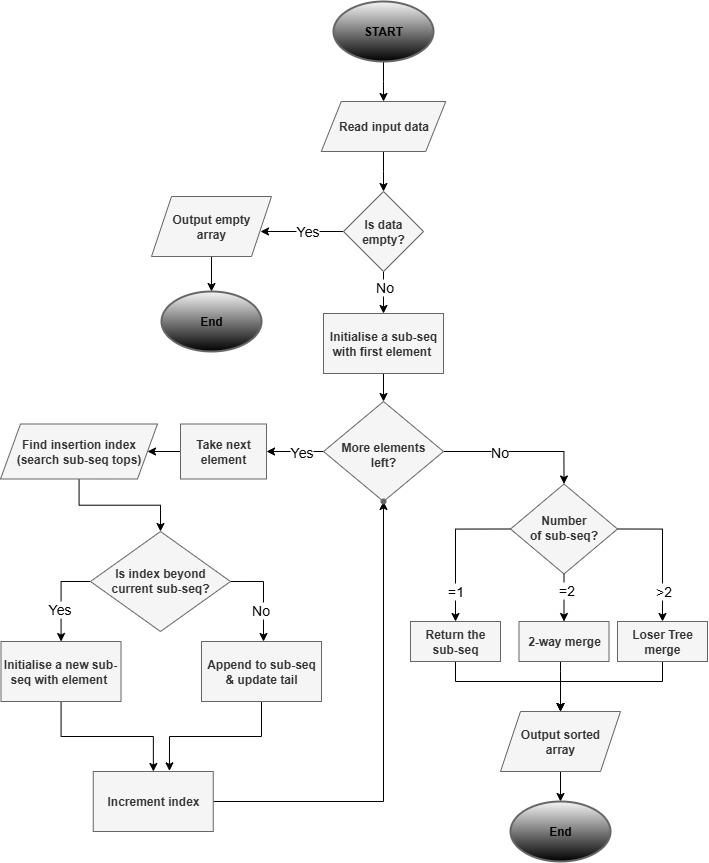
\includegraphics[width=6.41013in,height=7.73794in]{media/media/image2.jpg}
\section{Experimental Setup}\label{experimental-setup}

All experiments were executed on a 2020 MacBook Air featuring an Apple M1 8-core CPU and 8 GB of unified memory, running macOS 15.6.1. Implementations were compiled using Homebrew GCC 15 with C++20 and the following flags:
\[
\texttt{/opt/homebrew/bin/g++-15 -O3 -march=native -flto -funroll-loops -std=c++20}.
\]
All binaries were single-threaded and used only the compiler’s auto-vectorization (no explicit SIMD or parallelism).

\subsection{Algorithms Under Comparison}\label{algorithms-under-comparison}

\begin{itemize}
\item \textbf{LadderSort (this work):} deterministic two-phase ladder construction followed by adaptive merge (two-way galloping or \(K\)-way loser-tree).
\item \textbf{TimSort:} stable adaptive mergesort (we use \texttt{gfx::timsort}).
\item \textbf{QuickSort:} unstable in-place quicksort with three-way partitioning and median-of-three/ninther pivoting.
\item \textbf{IntroSort:} C++ \texttt{std::sort}.
\item \textbf{StableSort:} C++ \texttt{std::stable\_sort}.
\item \textbf{MergeSort:} reference top-down stable mergesort with a reusable buffer.
\end{itemize}
\section{\texorpdfstring{\textbf{Results and Discussion}}{Results and Discussion}}\label{results-and-discussion}

This section reports the empirical performance of LadderSort compared
with several baseline sorting algorithms under a range of input
distributions. For each workload, we sort arrays of 1 million, 10
million, and 100 million 32-bit integers. Each configuration (algorithm,
workload, size) is run 10 times; we report mean wall-clock time and
standard deviation. All algorithms are compiled with the same toolchain
and flags, and all runs are single-threaded. Correctness is verified
after every run using a standard sortedness check.

The algorithms compared are LadderSort (this work), TimSort, QuickSort
(our 3-way partition implementation), IntroSort (C++ \texttt{std::sort}),
StableSort (C++ \texttt{std::stable\_sort}), and a reference MergeSort
(top-down stable mergesort with reusable buffer). The workloads are:
uniform random, sorted ascending, sorted descending, band-limited almost-sorted
permutations, block-cyclic interleave, two-run riffle, social-feed
fan-in, and partial index merges.

\subsection{\texorpdfstring{\textbf{Uniform Random Inputs}}{Uniform Random Inputs}}\label{uniform-random-inputs}

The random generator produces 31-bit uniformly distributed integers with
duplicates possible but rare at these scales, so there is essentially no
exploitable order. All methods exhibit \(O(N\log N)\) behavior.

As expected, IntroSort (\texttt{std::sort}) is fastest on this workload due to
efficient in-place partitioning and good pivot selection. LadderSort
remains competitive but does not lead; with little structure to exploit,
Phase~1 generates many subsequences and the \(O(\log K)\) placement and merge
overhead becomes visible. StableSort and MergeSort move more data
because of merging and therefore typically trail IntroSort (and often
LadderSort). TimSort has no long runs to exploit and falls back to its
merge machinery, so it lags on pure random data. Table~1 summarizes the
timings for random inputs.

Table 1. Running time in seconds (mean \(\pm\) standard deviation over 10
runs) for uniform random inputs.

\begin{longtable}{@{}lrrr@{}}
\toprule
Name & 1M (s) & 10M (s) & 100M (s) \\
\midrule
\endfirsthead

\toprule
Name & 1M (s) & 10M (s) & 100M (s) \\
\midrule
\endhead

\bottomrule
\endfoot

\bottomrule
\endlastfoot

LadderSort & 0.060284 (\(\pm\)0.000284) & 0.711542 (\(\pm\)0.008003) & 8.352131 (\(\pm\)0.077906) \\
TimSort & 0.076062 (\(\pm\)0.000618) & 0.862810 (\(\pm\)0.000686) & 10.021459 (\(\pm\)0.064812) \\
QuickSort & 0.067775 (\(\pm\)0.000215) & 0.799014 (\(\pm\)0.000631) & 9.366719 (\(\pm\)0.132511) \\
IntroSort (C++) & 0.053926 (\(\pm\)0.000487) & 0.624150 (\(\pm\)0.000935) & 7.286278 (\(\pm\)0.079395) \\
StableSort (C++) & 0.061197 (\(\pm\)0.000084) & 0.712756 (\(\pm\)0.000536) & 8.397854 (\(\pm\)0.012043) \\
MergeSort & 0.067966 (\(\pm\)0.000106) & 0.775633 (\(\pm\)0.001740) & 9.244554 (\(\pm\)0.059223) \\
\end{longtable}

\subsection{\texorpdfstring{\textbf{Sorted Ascending Inputs}}{Sorted Ascending Inputs}}\label{sorted-ascending-inputs}

The sorted ascending generator returns an already sorted array,
essentially one long monotone run. Algorithms that detect and exploit
existing order are favored.

TimSort is the clear winner here: it detects a single run and finishes
in linear time with a very small constant factor. LadderSort is also
linear: Phase~1 places all elements into a single ladder (\(K=1\)) and
Phase~2 returns it directly. However, LadderSort pays some bookkeeping
and copy overhead, so it trails TimSort on this input. IntroSort and
QuickSort still perform partitioning work and remain roughly \(O(N\log N)\).
StableSort and MergeSort move more data than necessary and are also
slower than TimSort and LadderSort. Table~2 reports the results.

Table 2. Running time in seconds (mean \(\pm\) standard deviation over 10
runs) for sorted ascending inputs.

\begin{longtable}{@{}lrrr@{}}
\toprule
Name & 1M (s) & 10M (s) & 100M (s) \\
\midrule
\endfirsthead

\toprule
Name & 1M (s) & 10M (s) & 100M (s) \\
\midrule
\endhead

\bottomrule
\endfoot

\bottomrule
\endlastfoot

LadderSort & 0.003814 (\(\pm\)0.000779) & 0.032428 (\(\pm\)0.004184) & 0.412089 (\(\pm\)0.022985) \\
TimSort & 0.000308 (\(\pm\)0.000005) & 0.003213 (\(\pm\)0.000007) & 0.050807 (\(\pm\)0.002490) \\
QuickSort & 0.012358 (\(\pm\)0.000065) & 0.137529 (\(\pm\)0.000890) & 1.579520 (\(\pm\)0.010150) \\
IntroSort (C++) & 0.052283 (\(\pm\)0.000268) & 0.639582 (\(\pm\)0.001192) & 7.792178 (\(\pm\)0.030446) \\
StableSort (C++) & 0.007051 (\(\pm\)0.000022) & 0.083395 (\(\pm\)0.000275) & 0.977368 (\(\pm\)0.006558) \\
MergeSort & 0.006461 (\(\pm\)0.000016) & 0.085276 (\(\pm\)0.002955) & 1.008359 (\(\pm\)0.028363) \\
\end{longtable}

\subsection{\texorpdfstring{\textbf{Sorted Descending Inputs}}{Sorted Descending Inputs}}\label{sorted-descending-inputs}

The sorted descending generator produces a strictly descending array,
which is the adversarial edge case for LadderSort. Each new element is
smaller than all current tails, so Phase~1 creates a new ladder for
almost every element (\(K \approx N\)). The final \(K\)-way merge then costs
\(O(N\log N)\) with a large constant factor.

TimSort, by contrast, treats a descending sequence as a single run and
reverses it, resulting in linear time with a small constant. IntroSort
and QuickSort remain \(O(N\log N)\) but maintain good performance due to
robust pivoting. StableSort and MergeSort also perform well. Table~3
shows that sorted descending input exposes LadderSort's worst case,
while TimSort is effectively in its best case due to run detection and
reversal.

Table 3. Running time in seconds (mean \(\pm\) standard deviation over 10
runs) for sorted descending inputs.

{\small
\begin{longtable}{@{}lrrr@{}}
\toprule
Name & 1M (s) & 10M (s) & 100M (s) \\
\midrule
\endfirsthead

\toprule
Name & 1M (s) & 10M (s) & 100M (s) \\
\midrule
\endhead

\bottomrule
\endfoot

\bottomrule
\endlastfoot

LadderSort & 0.099664 (\(\pm\)0.000933) & 1.204596 (\(\pm\)0.028324) & 18.636188 (\(\pm\)1.049449) \\
TimSort & 0.000312 (\(\pm\)0.000003) & 0.003314 (\(\pm\)0.000022) & 0.040585 (\(\pm\)0.000256) \\
QuickSort & 0.012717 (\(\pm\)0.000089) & 0.140608 (\(\pm\)0.004181) & 1.595088 (\(\pm\)0.004581) \\
IntroSort (C++) & 0.007342 (\(\pm\)0.000009) & 0.094218 (\(\pm\)0.014076) & 0.998968 (\(\pm\)0.001724) \\
StableSort (C++) & 0.008605 (\(\pm\)0.000032) & 0.100982 (\(\pm\)0.000412) & 1.152614 (\(\pm\)0.002390) \\
MergeSort & 0.009635 (\(\pm\)0.000030) & 0.108443 (\(\pm\)0.002083) & 1.279382 (\(\pm\)0.015677) \\
\end{longtable}
}

\subsection{\texorpdfstring{\textbf{Nearly Sorted Inputs with Bounded Local Jitter}}{Nearly Sorted Inputs with Bounded Local Jitter}}\label{nearly-sorted-inputs-with-bounded-local-jitter}

In the band-limited permutation workload, we start from the sorted
sequence \(1,\ldots,N\) and shuffle only within windows of size \(W+1\)
(here \(W=32\)). No element moves more than 32 positions. This keeps the
number of nondecreasing subsequences effectively small (\(K \approx W+1\)),
which is where LadderSort's \(O(N\log K)\) behavior is advantageous.

In Phase~1, LadderSort quickly finds the correct ladder using its hinted
search; in Phase~2, it merges only a few ladders, not hundreds or
thousands. The measurements show that LadderSort is fastest across
sizes, with StableSort close behind due to cache-friendly sequential
merges. TimSort benefits from local order but cannot rely on a single
long run; its stack of short runs induces more merging work, so it
trails LadderSort and often StableSort. Partition-based methods
(IntroSort and QuickSort) do not exploit the small \(K\) and remain
\(O(N\log N)\). Table~4 presents the results.

Table 4. Running time in seconds (mean \(\pm\) standard deviation over 10
runs) for band-limited, nearly sorted inputs (\(W=32\)).

{\small
\begin{longtable}{@{}lrrr@{}}
\toprule
Name & 1M (s) & 10M (s) & 100M (s) \\
\midrule
\endfirsthead

\toprule
Name & 1M (s) & 10M (s) & 100M (s) \\
\midrule
\endhead

\bottomrule
\endfoot

\bottomrule
\endlastfoot

LadderSort & 0.018413 (\(\pm\)0.001220) & 0.184734 (\(\pm\)0.002650) & 1.928484 (\(\pm\)0.041110) \\
TimSort & 0.025139 (\(\pm\)0.000041) & 0.247422 (\(\pm\)0.001032) & 2.519951 (\(\pm\)0.011741) \\
QuickSort & 0.027009 (\(\pm\)0.000091) & 0.291233 (\(\pm\)0.001167) & 3.145271 (\(\pm\)0.009378) \\
IntroSort (C++) & 0.056191 (\(\pm\)0.000062) & 0.677812 (\(\pm\)0.002503) & 7.974671 (\(\pm\)0.045230) \\
StableSort (C++) & 0.018900 (\(\pm\)0.000038) & 0.198993 (\(\pm\)0.000408) & 2.141182 (\(\pm\)0.008664) \\
MergeSort & 0.023829 (\(\pm\)0.000098) & 0.234845 (\(\pm\)0.001104) & 2.684934 (\(\pm\)0.022102) \\
\end{longtable}
}

\subsection{\texorpdfstring{\textbf{Block-Cyclic Interleave}}{Block-Cyclic Interleave}}\label{block-cyclic-interleave}

The block-cyclic interleave workload models bursty fan-in from a few
already sorted producers. Here \(K=8\) sources emit small sorted blocks of
size \(B=4\) in round-robin order, so the global sequence is a weave of
eight monotone subsequences.

LadderSort aligns almost perfectly with this structure. Phase~1 assigns
each element to one of approximately \(K\) ladders using the hinted search,
and Phase~2 performs a light \(K\)-way merge. As a result, LadderSort is
fastest across all sizes. TimSort benefits from local sortedness but
observes many short runs rather than a single long run, so its merge
stack performs more work. StableSort is competitive but pays extra
copying. Partition-based methods ignore the small-\(K\) structure and stay
in \(O(N\log N)\) territory. Table~5 shows the timing results.

Table 5. Running time in seconds (mean \(\pm\) standard deviation over 10
runs) for block-cyclic interleave inputs (\(K=8, B=4\)).

{\small
\begin{longtable}{@{}lrrr@{}}
\toprule
Name & 1M (s) & 10M (s) & 100M (s) \\
\midrule
\endfirsthead

\toprule
Name & 1M (s) & 10M (s) & 100M (s) \\
\midrule
\endhead

\bottomrule
\endfoot

\bottomrule
\endlastfoot

LadderSort & 0.009034 (\(\pm\)0.001325) & 0.087689 (\(\pm\)0.003280) & 0.954970 (\(\pm\)0.035121) \\
TimSort & 0.011258 (\(\pm\)0.000115) & 0.114428 (\(\pm\)0.008528) & 1.084507 (\(\pm\)0.017320) \\
QuickSort & 0.048795 (\(\pm\)0.000060) & 0.545557 (\(\pm\)0.001485) & 6.361478 (\(\pm\)0.019182) \\
IntroSort (C++) & 0.037141 (\(\pm\)0.000164) & 0.428570 (\(\pm\)0.000647) & 4.776093 (\(\pm\)0.019065) \\
StableSort (C++) & 0.009841 (\(\pm\)0.000054) & 0.114720 (\(\pm\)0.000686) & 1.331516 (\(\pm\)0.009939) \\
MergeSort & 0.011499 (\(\pm\)0.000085) & 0.128904 (\(\pm\)0.000871) & 1.565909 (\(\pm\)0.025747) \\
\end{longtable}
}

\subsection{\texorpdfstring{\textbf{Two-Run Riffle}}{Two-Run Riffle}}\label{two-run-riffle}

The two-run riffle workload interleaves two already sorted halves by
coin flip, so the data effectively decomposes into about two monotone
subsequences (\(K \approx 2\)).

LadderSort is well matched to this pattern. Phase~1 reconstructs the two
ladders, and Phase~2 reduces them via a single two-way galloping merge.
LadderSort therefore leads at all sizes. TimSort comes next; the
frequent alternation prevents it from exploiting a single long run and
increases merge bookkeeping. StableSort and MergeSort are close because
they perform the appropriate two-way merge work but with more buffer
traffic. Partition-based methods do not benefit from the small \(K\) and
remain significantly slower. Table~6 lists the measured times.

Table 6. Running time in seconds (mean \(\pm\) standard deviation over 10
runs) for two-run riffle inputs.

{\small
\begin{longtable}{@{}lrrr@{}}
\toprule
Name & 1M (s) & 10M (s) & 100M (s) \\
\midrule
\endfirsthead

\toprule
Name & 1M (s) & 10M (s) & 100M (s) \\
\midrule
\endhead

\bottomrule
\endfoot

\bottomrule
\endlastfoot

LadderSort & 0.011840 (\(\pm\)0.000138) & 0.115206 (\(\pm\)0.003219) & 1.339615 (\(\pm\)0.033321) \\
TimSort & 0.016426 (\(\pm\)0.000408) & 0.153702 (\(\pm\)0.000894) & 1.611879 (\(\pm\)0.022445) \\
QuickSort & 0.041296 (\(\pm\)0.000216) & 0.496247 (\(\pm\)0.001000) & 5.322729 (\(\pm\)0.019506) \\
IntroSort (C++) & 0.040121 (\(\pm\)0.000162) & 0.459920 (\(\pm\)0.000465) & 4.595198 (\(\pm\)0.032761) \\
StableSort (C++) & 0.013342 (\(\pm\)0.000316) & 0.143149 (\(\pm\)0.000607) & 1.619594 (\(\pm\)0.020108) \\
MergeSort & 0.014821 (\(\pm\)0.000096) & 0.161039 (\(\pm\)0.001319) & 1.927994 (\(\pm\)0.048978) \\
\end{longtable}
}

\subsection{\texorpdfstring{\textbf{Social-Feed Fan-In}}{Social-Feed Fan-In}}\label{social-feed-fan-in}

The social-feed fan-in workload approximates a per-user feed where
10--40 followees emit in sticky bursts. Timestamps often repeat and
advance only by small increments, producing a small number of ladders
(small \(K\)) and large tie plateaus. This is essentially a streaming \(K\)-way
merge problem.

LadderSort matches this shape closely. Phase~1 reconstructs the
per-source ladders, and the \(K\)-way loser-tree merge in Phase~2 outputs
the global minimum using a deterministic tie-breaking rule. LadderSort therefore
leads across sizes. TimSort benefits from local runs but pays more
overhead for run detection and frequent merges. StableSort tracks
LadderSort within about 20--40\%, and MergeSort follows behind, as both
perform appropriate merge work on tie-heavy inputs. QuickSort and
IntroSort do not benefit from the small \(K\) or the ties; partitioning
large equality plateaus is costly. Table~7 gives the timings.

Table 7. Running time in seconds (mean \(\pm\) standard deviation over 10
runs) for social-feed fan-in inputs.

{\small
\begin{longtable}{@{}lrrr@{}}
\toprule
Name & 1M (s) & 10M (s) & 100M (s) \\
\midrule
\endfirsthead

\toprule
Name & 1M (s) & 10M (s) & 100M (s) \\
\midrule
\endhead

\bottomrule
\endfoot

\bottomrule
\endlastfoot

LadderSort & 0.010511 (\(\pm\)0.001152) & 0.101416 (\(\pm\)0.005685) & 1.112252 (\(\pm\)0.030992) \\
TimSort & 0.017365 (\(\pm\)0.000147) & 0.148320 (\(\pm\)0.002117) & 1.589728 (\(\pm\)0.011485) \\
QuickSort & 0.013070 (\(\pm\)0.000044) & 0.154958 (\(\pm\)0.000549) & 1.841403 (\(\pm\)0.017027) \\
IntroSort (C++) & 0.022060 (\(\pm\)0.000046) & 0.623835 (\(\pm\)0.001309) & 9.208073 (\(\pm\)0.084188) \\
StableSort (C++) & 0.013298 (\(\pm\)0.000116) & 0.142700 (\(\pm\)0.000788) & 1.631445 (\(\pm\)0.020788) \\
MergeSort & 0.013936 (\(\pm\)0.000139) & 0.155518 (\(\pm\)0.000805) & 1.863321 (\(\pm\)0.035130) \\
\end{longtable}
}

\subsection{\texorpdfstring{\textbf{Partial Index Merges}}{Partial Index Merges}}\label{partial-index-merges}

The partial index merge workload models merging a handful of hot
posting-list segments whose docID ranges overlap. Many equal keys appear
across segments, and items arrive in short bursts. This is again a
small-\(K\) streaming merge.

LadderSort is well aligned with this structure. Phase~1 recovers the
per-segment ladders, and the \(K\)-way loser tree in Phase~2 streams the
global minimum using a deterministic tie-breaking rule. LadderSort leads across
sizes. TimSort is the next best method: it benefits from local runs but
pays more for run detection and repeated merges. StableSort and
MergeSort remain reasonably close but suffer from heavier buffer
traffic. Partition-based methods do not benefit from ties or small \(K\) and
spend time partitioning large equality plateaus. Table~8 shows the
performance.

Table 8. Running time in seconds (mean \(\pm\) standard deviation over 10
runs) for partial index merge inputs.

{\small
\begin{longtable}{@{}lrrr@{}}
\toprule
Name & 1M (s) & 10M (s) & 100M (s) \\
\midrule
\endfirsthead

\toprule
Name & 1M (s) & 10M (s) & 100M (s) \\
\midrule
\endhead

\bottomrule
\endfoot

\bottomrule
\endlastfoot

LadderSort & 0.010009 (\(\pm\)0.001179) & 0.098894 (\(\pm\)0.002472) & 1.186517 (\(\pm\)0.074247) \\
TimSort & 0.016116 (\(\pm\)0.000091) & 0.147210 (\(\pm\)0.009107) & 1.580356 (\(\pm\)0.028986) \\
QuickSort & 0.028305 (\(\pm\)0.000063) & 0.316342 (\(\pm\)0.007865) & 3.589427 (\(\pm\)0.032215) \\
IntroSort (C++) & 0.026411 (\(\pm\)0.000094) & 0.306428 (\(\pm\)0.000769) & 3.212840 (\(\pm\)0.010319) \\
StableSort (C++) & 0.017223 (\(\pm\)0.000027) & 0.182740 (\(\pm\)0.000493) & 2.026903 (\(\pm\)0.012580) \\
MergeSort & 0.017828 (\(\pm\)0.000050) & 0.195492 (\(\pm\)0.002226) & 2.182471 (\(\pm\)0.018061) \\
\end{longtable}
}

Overall, the picture is consistent across sizes and workloads.
LadderSort is at its best when the input decomposes into a small number
of interleaved nondecreasing streams (small \(K\)): block-cyclic interleave,
two-run riffle, social-feed fan-in, and partial-index merges all favor
its hinted placement plus \(K\)-way loser-tree merge, with deterministic tie-handling
benefiting tie-heavy cases. It is competitive---but not leading---on uniform
random, where there's little structure to exploit and partition-based
\texttt{std::sort} sets the pace. At the other extreme, fully monotone inputs
split: TimSort wins outright on both sorted and reverse-sorted data
thanks to run detection (and reversal), while LadderSort remains linear
on ascending but hits its worst case on descending as \(K \approx N\). Stable
baselines (\texttt{std::stable\_sort} and our mergesort) track closely on
merge-friendly workloads but pay extra memory traffic and generally sit
behind LadderSort there. The takeaway is practical: use LadderSort when
your pipeline naturally produces a few ordered sources or bounded-jitter
streams; reach for TimSort on long runs (including descending), and
prefer \texttt{std::sort} when inputs look unstructured.

\subsection{\texorpdfstring{\textbf{Asymptotic Behavior and Structural Interpretation}}{Asymptotic Behavior and Structural Interpretation}}\label{asymptotic-behavior-and-structural-interpretation}

The empirical results above are consistent with the theoretical analysis
of LadderSort in terms of \(N\) (input length) and \(K\) (number of
nondecreasing subsequences produced in Phase~1).

Phase~1 places each key into the leftmost ladder whose tail is less than
or equal to the key. Tails are kept in a non-increasing \texttt{tops} array. Each
placement performs a hinted lookup that uses a local probe, an
exponential gallop to bound the search region, and a binary search
within that region. The amortized cost per element is \(O(\log K)\), so Phase~1
is \(O(N\log K)\).

Phase~2 merges the \(K\) ladders. If \(K=1\), the single ladder is returned in
\(O(N)\). If \(K=2\), a two-way galloping merge costs \(O(N)\). For \(K>2\), a
loser-tree merge over \(K\) runs costs \(O(K)\) to build the tree and \(O(\log K)\)
per extract-and-advance step, for a total of \(O(N\log K)\). Combining both
phases yields
\[
T(N,K)=O(N\log K + K),
\]
which is \(\Theta(N)\) when \(K=1\) and \(\Theta(N\log K)\) when \(K\ge 2\). The additive
\(K\) term is dominated by \(N\log K\) whenever \(N\ge K\). Table~9 summarizes the
parametric bounds.

Table 9. Parametric bounds for LadderSort in terms of \(N\) and \(K\).

{\small
\begin{longtable}{@{}p{0.14\linewidth}p{0.22\linewidth}p{0.18\linewidth}p{0.42\linewidth}@{}}
\toprule
Notation & Time bound & Valid when & Interpretation \\
\midrule
\endfirsthead

\toprule
Notation & Time bound & Valid when & Interpretation \\
\midrule
\endhead

\bottomrule
\endfoot

\bottomrule
\endlastfoot

Big-O & \(O(N\log K + K)\) & All \(K\ge 1\) & Placement + loser-tree merge; \(+K\) is tree build. \\
Big-Theta & \(\Theta(N)\) & \(K=1\) & Single run; scan and return. \\
 & \(\Theta(N\log K)\) & \(K\ge 2\) & Tight bound when merging \(K\) runs. \\
Big-Omega & \(\Omega(N)\) & All \(K\) & Must at least read/output \(N\) items. \\
Little-o & \(o(N\log N)\) & \(K=N^{o(1)}\) (e.g., \(K=O((\log N)^c)\)) & Strictly sub-\(N\log N\) when \(K\) grows sub-polynomially. \\
Little-omega & \(\omega(N)\) & \(K\to\infty\) & Superlinear whenever \(K\) diverges. \\
Space & \(O(N+K)\) &  & Linear buffer for runs/output + \(O(K)\) metadata. \\
\end{longtable}
}

These bounds explain the trends observed in the workloads:
\begin{itemize}
\item Best case: already sorted or all keys equal. Here \(K=1\) and \(T(N,1)=\Theta(N)\); this matches the linear behavior seen on sorted ascending inputs.
\item Small-\(K\) inputs: constant or polylogarithmic \(K\) (for example, block-cyclic, two-run riffle, social-feed fan-in, and partial index merges). In these cases, \(T(N,K)\) is \(\Theta(N)\) or \(\Theta(N\log\log N)\), which is strictly below \(N\log N\); the measurements confirm that LadderSort is faster than partition-based baselines and competitive with or better than merge-based baselines.
\item Random permutations: for distinct keys, classical patience-sorting theory implies that the minimum number of nondecreasing subsequences equals the length of the longest decreasing subsequence, which is \(\Theta(\sqrt{N})\) in expectation. Thus \(K\approx \Theta(\sqrt{N})\) and the expected running time is about \(\tfrac{1}{2}\Theta(N\log N)\), consistent with LadderSort being competitive but not leading on uniform random inputs.
\item Adversarial descending: every element starts a new ladder, \(K=N\), and \(T(N,N)=\Theta(N\log N)\). This matches the worst-case behavior measured on sorted descending inputs.
\end{itemize}

Table 10 connects representative input families from the experiments to
typical \(K\) and resulting complexity.

Table 10. Representative inputs, typical \(K\), and resulting complexity for
LadderSort.

{\small
\begin{longtable}{@{}p{0.30\linewidth}p{0.12\linewidth}p{0.18\linewidth}p{0.36\linewidth}@{}}
\toprule
Input family (from Results) & Typical \(K\) & Time & Notes \\
\midrule
\endfirsthead

\toprule
Input family (from Results) & Typical \(K\) & Time & Notes \\
\midrule
\endhead

\bottomrule
\endfoot

\bottomrule
\endlastfoot

Sorted ascending & 1 & \(\Theta(N)\) & Phase~1 makes one run; Phase~2 returns it. \\
Two-run riffle & \(\approx 2\) & \(\Theta(N)\) & Collapses via one 2-way galloping merge. \\
Block-cyclic (\(K=8, B=4\)) & 8 & \(\Theta(N\log 8)\) & Few long runs; hinted placement is cheap. \\
Band-limited jitter (\(W=32\)) & \(\le 33\) & \(\Theta(N\log 33)\) & Local disorder; small effective \(K\). \\
Social-feed fan-in (10--40 src) & 10--40 & \(\Theta(N\log K)\) & Tie-heavy; deterministic tie-breaking ensures reproducible output. \\
Search-index partial merges (\(K=16\)) & 16 & \(\Theta(N\log 16)\) & Overlap and bursts across runs. \\
Uniform random (distinct keys) & \(\Theta(\sqrt{N})\) & \(\Theta(N\log \sqrt{N})\) & Classic behavior. \\
Strictly descending & \(N\) & \(\Theta(N\log N)\) & Worst case (run explosion). \\
All keys equal & 1 & \(\Theta(N)\) & Ties collapse into one run. \\
\end{longtable}
}

Overall, the results demonstrate that LadderSort's running time scales
primarily with the effective structure parameter \(K\) rather than with \(N\)
alone. The algorithm attains linear time on fully sorted and tie-heavy
small-\(K\) workloads, remains strictly sub-\(N\log N\) whenever \(K\) is small,
behaves close to half-height \(N\log N\) on random permutations, and
degrades gracefully to \(N\log N\) on adversarial descending inputs.

\section{\texorpdfstring{\textbf{Limitations and Threats to
Validity}}{Limitations and Threats to Validity}}\label{limitations-and-threats-to-validity}

\subsection{\texorpdfstring{\textbf{Algorithmic
Limitations}}{Algorithmic Limitations}}\label{algorithmic-limitations}

The performance of LadderSort depends critically on the number of
subsequences K discovered in Phase 1. For adversarial inputs where K is
approximately N (for example, strictly descending sequences with few
ties), the algorithm degrades to Theta(N log N) with a larger constant
factor than highly tuned in-place sorts, because it must materialize
many ladders and then perform a K-way merge. LadderSort is not in-place:
it uses O(N + K) auxiliary space, which can be problematic when memory
is constrained. In addition, run construction may touch many ladders in
quick succession; when K is large this increases write scattering and
may harm cache locality compared with contiguous two-way merges.
Finally, the analysis and implementation assume a total order and deterministic tie-breaking for equal keys. Domains with non-total comparators (for example, floating-point NaNs) or very expensive comparisons/key extraction may change the practical trade-offs.

\subsection{\texorpdfstring{\textbf{Workload
Representativeness}}{Workload Representativeness}}\label{workload-representativeness}

The synthetic generators are designed to capture common systems patterns
(nearly sorted data with local jitter, block-cyclic fan-in, two-run
riffles, social-feed fan-in, and partial index merges), but they cannot
cover the full diversity of real workloads. Specific parameter choices
(for example, W = 32, K in \{8, 16, 24\}, burst sizes) may favor some
algorithms; different settings could shift the relative ranking. The
benchmarks use only 32-bit integer keys; behavior with strings,
composite keys, or custom comparators may differ due to larger key
sizes, pointer indirection, and different cache behavior. Although a
uniform-random baseline is included, the study does not explore all
pathological patterns (for example, alternating high/low sequences
engineered to maximize K, or inputs tuned specifically to stress
galloping thresholds).

\subsection{\texorpdfstring{\textbf{Implementation
Comparability}}{Implementation Comparability}}\label{implementation-comparability}

The quicksort and mergesort baselines are competent, single-file
reference implementations; highly engineered library versions may behave
differently. The TimSort baseline is taken from a specific header-only
implementation, and other TimSort variants (with different run bounds,
stack policies, or gallop thresholds) may perform better or worse. The
behavior of std::sort and std::stable\_sort depends on the standard
library and allocator; the reported results reflect libstdc++ on an
arm64 platform. LadderSort and the reference mergesort reuse scratch
buffers across runs; despite a warm-up iteration for each algorithm,
differences in allocation strategy or buffer-reuse policies can still
influence performance.

\subsection{\texorpdfstring{\textbf{Construct Validity of
Measurements}}{Construct Validity of Measurements}}\label{construct-validity-of-measurements}

The evaluation reports only wall-clock time. We do not measure memory
usage, peak footprint, bandwidth, or microarchitectural counters (for
example, cache, TLB, or branch behavior). Some algorithms move less data
(in-place methods) or exhibit better locality on particular inputs; such
advantages are not fully captured by timing alone. Energy consumption is
also not measured, even though it is increasingly relevant for mobile,
embedded, and edge platforms.

\subsection{\texorpdfstring{\textbf{Reproducibility and External
Validity}}{Reproducibility and External Validity}}\label{reproducibility-and-external-validity}

The experiments use fixed random seeds, a documented compile command,
and a post-run correctness check, which supports reproducibility on the
same platform and toolchain. Nevertheless, small code or toolchain
changes (for example, inlining decisions or link-time optimization
partitioning) can alter constant factors. Cross-platform reproducibility
will require rebuilding with native compilers and libraries, and results
may still vary due to different ABIs, standard libraries, and allocator
behavior.

\subsection{\texorpdfstring{\textbf{Mitigations and Future
Directions}}{Mitigations and Future Directions}}\label{mitigations-and-future-directions}

Several of these threats can be mitigated in future work. Extending the
evaluation to additional data types, key distributions, and adversarial
patterns would strengthen claims about generality. Porting the
implementation to multiple platforms and standard-library stacks, and
reporting memory and microarchitectural metrics alongside time, would
provide a more complete performance profile. On the algorithmic side,
exploring in-place or more memory-efficient variants of LadderSort, as
well as mechanisms to detect when K becomes large and switch to
alternative strategies, could reduce the impact of its worst-case
regimes.

\section{\texorpdfstring{\textbf{Conclusions and Future
Work}}{Conclusions and Future Work}}\label{conclusions-and-future-work}

We introduced LadderSort, a deterministic adaptive sorting algorithm whose running time depends on the number \(K\) of interleaved nondecreasing subsequences present in the input. The analysis characterizes performance in terms of N, the input length, and K, the number of subsequences produced in Phase 1: T(N, K) is Theta(N) when K = 1 and Theta(N log K) otherwise, with linear space plus an additional O(K) metadata footprint. This parameterization matches what we observe in practice: the running time tracks the amount of order already present in the data rather than assuming fully random inputs.

Across a suite of workloads that mirror real systems band-limited
``nearly sorted'' data, block-cyclic fan-in, two-run riffles,
social-feed assembly, and partial index merges LadderSort consistently
benefits from small K. It remains competitive on uniform random inputs
and clearly leads when existing order is concentrated in a few
interleaved streams, while degrading gracefully to N log N on
adversarial descending inputs. The algorithm behaves deterministically under duplicates, emitting equal keys in a fixed ladder-identifier order in tie-heavy scenarios that arise in feed construction and index maintenance. Where other methods excel on specific shapes (for example, TimSort on fully sorted or reversed arrays via run detection and reversal), LadderSort remains close in those linear regimes and surpasses partition-based baselines on small-K interleaves.

Methodologically, LadderSort achieves these results using simple
building blocks: a hinted search over a nonincreasing array of run tails
for element placement, a two-way galloping merge when K = 2, and a
loser-tree merge when K \textgreater{} 2. The design avoids heavy data
structures, is straightforward to implement, and scales to very large
inputs without tuning beyond standard compiler optimizations.

There are several natural directions for future work. On the theory
side, tighter distributional analyses of K under realistic data models
(including duplicates and correlations) would sharpen the expected-time
guarantees. On the systems side, cache-aware and reduced-copy variants,
as well as parallel and external-memory versions, could broaden the
algorithm's applicability in large-scale and resource-constrained
environments. Finally, adaptive switching strategies detecting when K
becomes large or when a single long run dominates and then falling back
to existing library sorts could provide near best-of-both-worlds
behavior automatically. In this way, LadderSort can serve as a bridge
between worst-case-oriented designs and the partial order that dominates
many real-world data streams, offering a simple, deterministic alternative that is fast precisely where many practical workloads lie.
\section{References}\label{references}

{[}1{]} Knuth, D.E. \emph{The Art of Computer Programming; Volume 3: Sorting and Searching}; 2nd ed.; Addison-Wesley: Reading, MA, USA, 1998.

{[}2{]} Dijkstra, E.W. Smoothsort, an alternative for sorting in situ. EWD 796, 1981.

{[}3{]} Auger, N.; Jugé, V.; Nicaud, C.; Pivoteau, C. On the Worst-Case Complexity of TimSort. In \emph{Proceedings of ESA 2018}; LIPIcs, Volume 112; pp. 4:1--4:13.

{[}4{]} Munro, J.I.; Wild, S. Nearly-Optimal Mergesorts: Fast, Practical Sorting Methods That Excel on Partially Ordered Data. In \emph{Proceedings of ESA 2018}; extended manuscript.

{[}5{]} Cawley Gelling, W.; Nebel, M.E.; Smith, B.; Wild, S. Multiway PowerSort. arXiv 2023, arXiv:2209.06909.

{[}6{]} Jugé, V. Adaptive Shivers Sort: An Alternative Sorting Algorithm. arXiv 2018, arXiv:1809.08411; see also SIAM publication (2020).

{[}7{]} Mannila, H. Measures of Presortedness and Optimal Sorting Algorithms. \emph{IEEE Trans. Comput.} 1985, C-34, 318--325.

{[}8{]} Estivill-Castro, V.; Wood, D. A Survey of Adaptive Sorting Algorithms. \emph{ACM Comput. Surv.} 1992, 24, 441--476.

{[}9{]} Skiena, S.S. Encroaching Lists as a Measure of Presortedness. \emph{BIT Numer. Math.} 1988, 28, 775--784.

{[}10{]} Fredman, M.L. On Computing the Length of Longest Increasing Subsequences. \emph{Discrete Math.} 1975, 11, 29--35.

{[}11{]} Dilworth, R.P. A Decomposition Theorem for Partially Ordered Sets. \emph{Ann. Math.} 1950, 51, 161--166.

{[}12{]} Aldous, D.; Diaconis, P. Longest Increasing Subsequences: From Patience Sorting to the Baik--Deift--Johansson Theorem. \emph{Bull. Am. Math. Soc.} 1999, 36, 413--432.

{[}13{]} K-way Merge Algorithm. Wikipedia. Available online: \url{https://en.wikipedia.org/wiki/K-way_merge_algorithm} (accessed on October 2025).

{[}14{]} Polyntsov, M.; Grigorev, V.; Smirnov, K.; Chernishev, G. Implementing the Comparison-Based External Sort. arXiv 2022, arXiv:2207.12713.

{[}15{]} Edelkamp, S.; Weiß, A. BlockQuicksort: Avoiding Branch Mispredictions in Quicksort. In \emph{Proceedings of ESA 2016}; LIPIcs, Volume 57; pp. 38:1--38:16.

{[}16{]} Peters, O.R.L. Pattern-Defeating Quicksort. arXiv 2021, arXiv:2106.05123.

{[}17{]} Knuth, D.E. \emph{The Art of Computer Programming; Volume 3: Sorting and Searching}; 2nd ed.; Addison-Wesley: Reading, MA, USA, 1998; Sections 5.4--5.5.

{[}18{]} Edelkamp, S.; Elmasry, A.; Katajainen, J. Adaptive Heapsort: Source Code. Department of Computer Science, University of Copenhagen, Technical Report (CPH STL Report 2011-1), 2012.

{[}19{]} Vitter, J.S. External Memory Algorithms and Data Structures: Dealing with MASSIVE Data. \emph{ACM Computing Surveys}, 2001.

\end{document}